\documentclass{article}
% Catheter to guidewire

\usepackage[english]{babel}
\usepackage{subcaption}
\usepackage{makecell}
\usepackage{pdfpages}
\bibliographystyle{vancouver}

% Set page size and margins
% Replace `letterpaper' with `a4paper' for UK/EU standard size
\usepackage[letterpaper,top=2cm,bottom=2cm,left=3cm,right=3cm,marginparwidth=1.75cm]{geometry}

% Useful packages
\usepackage{amsmath}
\usepackage{graphicx}
\usepackage[colorlinks=true, allcolors=blue]{hyperref}

\title{Project Plan: Real-Time 3D detection and localization of passive guidewire using MRI for the CathBot platform }
\author{Martin Reinok}

\begin{document}
\maketitle

% Table of Contents
\tableofcontents
\newpage

\section{Introduction}
% Risk of infection
Cardiovascular diseases remain as a predominant cause of global mortality, motivating the exploration of alternative medical interventions to open surgery, which has higher odds of mortality and complications. An viable alternative has been endovascular operation, which primary benefit is faster recovery due to the minimally invasive approach. Normally, the endovascular operation is performed with the help of Computed Tomography (CT) imaging, which involves the use of x-rays - a form of ionizing radiation that increases the risk of cancer. An alternative to CT is the use of Magnetic Resonance Imaging (MRI) technology, which is more expensive to use, but does not involve any ionizing radiation and has the potential for better quality imaging compared to CT. The CathBot project \cite{cathbot} proposes MR-safe teleoperation platform to manipulate endovascular instrumentation remotely and to provide operators with haptic feedback for endovascular tasks. This thesis focuses on addressing the shortcomings of MRI for endovascular operations by implementing guidewire detection and safety layers to ensure patient protection for CathBot operation. The safety layers will be integrated on the CathBot using haptic feedback capabilities, which inform the operator of potential issues.

\section{Background}
\textit{Here should be a "Background" section that explains the components used in this project. 
\\ The components are the following:}
\begin{itemize}
    \item MRI
    \item Fluoroscopy briefly
    \item Guidewire and catheter
    \item Computer Vision briefly
    \item CNN and DNN
\end{itemize}

\section{Related Work and Research}
Currently, fluoroscopy is the standard imaging method for minimally invasive endovascular procedures due to it's real-time capabilities, as well as good resolution. However fluoroscopy coincides with radiation exposure both to the patient and the doctor and it requires injection of contrast agents to be able to see veins or arteries \cite{pmid35420239}. Many commercial robotic interfaces exist for fluoroscopy-based procedures, such as the CorPath GRX platform (Corindus, a Siemens Healthineers Company, Watham, MA, USA), however most commercial robotic solutions based on MRI are still in the works, such as CathBot \cite{cathbot} or Nano4Imaging's \textit{TRACKR AI software} \cite{nano4imaging}. Nano4Imaging have manufactured their own passive guidewire and developed CNN-based tracking software for it \textcolor{red}{(find a citation)}.

MRI-guided endovascular intervention is an emerging field of study due to the many benefits it provides, including high-contrast visualization of vessel walls, multiplanar/3D capabilities and reduced exposure to radiation compared to fluoroscopy \cite{active-vs-passive-tracking}. Using robotic methods for endovascular intervention also provides the benefit of precision and stability \cite{pmid24663088}. The majority of current experimental MRI-guided endovascular interventions deem MRI as a feasible alternative to fluoroscopy, however in-vivo studies are sparse \cite{pmid35420239}. The main shortcomings of MRI-usage for guidewire guidance have been reported as the following, based on overview of 43 experiments \cite{pmid35420239}:

\begin{itemize}
    \item Low temporal/spatial resolution (17/43 articles)
    \item Guidewire/catheter visibility (14/43 articles)
    \item Safety (13/43 articles)
    \item Manual MRI slice alignment (7/43 articles) 
\end{itemize}

This thesis will aim to improve the \textit{Guidewire visibility}, \textit{Safety} and \textit{MRI slice alignment} issues by implementing a software layer on top of the CathBot robotic platform \cite{cathbot}.\\

\textbf{Low temporal/spatial resolution} is a fundamental MRI limitation, there must be a tradeoff between spatial resolution, temporal resolution and signal-to-noise(SNR) ratio \cite{real-time-mri}. MRI does have a reputation for being slow, especially compared to x-ray and fluoroscopy, which can achieve 7.5 to 15 images per second \cite{pmid25208902}. The speed of MRI is limited by the nuclear magnetic resonance (NMR) relaxation \cite{real-time-mri}, meaning images can not be taken faster than the nucleus relaxation time after magnetic pulse.
\\
However modern MRI sequences such as spoiled Gradient-Recalled-Echo (GRE) and balanced Steady-State Free Precession (bSSFP) can provide adequate resolution at real-time speeds \cite{real-time-mri}. Out of the two sequences, bSSFP is generally preferred, as it provides a higher SNR than GRE, but as a downside it has off-resonance effects \cite{bssfp-vs-gre-mri}. Both, the SNR and off-resonance effects have been demonstrated in \autoref{fig:gre-bssfp-example}.

\begin{figure}[h]
    \centering
    \begin{minipage}{0.45\textwidth}
        \centering
        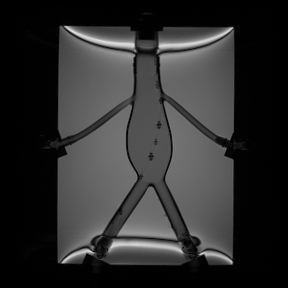
\includegraphics[width=\textwidth]{img/bssfp-example.jpg}
        \subcaption{}
        \label{fig:bssfp-example}
    \end{minipage}\hfill
    \begin{minipage}{0.45\textwidth}
        \centering
        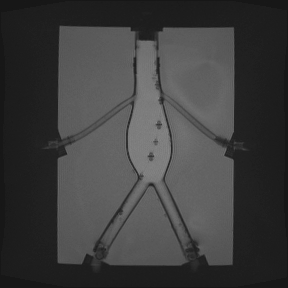
\includegraphics[width=\textwidth]{img/gre-example.jpg}
        \subcaption{}
        \label{fig:gre-example}
    \end{minipage}
    \caption{\textbf{a)} bSSFP sequence with visible off-resonance effects on the top and bottom. \textbf{b)} GRE sequence with no noticeable resonance effects, however the SNR is lower compared to the bSSFP sequence. \textit{Images taken at the University of Twente of the aneurysm phantom} }
    \label{fig:gre-bssfp-example}
\end{figure}

\textbf{Guidewire visibility} is directly related to the resolution of the image, if a MRI real-time equivalent sequence is used, the guidewire and/or catheter is often not visible, unless an active guidewire is used. Active guidewire requires to be connected to a voltage source and additional software for detection, which makes this very costly compared to using a passive guidewire. Passive tracking uses embedded steel markers that create susceptibility artifacts under MR. An example of passive guidewire with markers can be seen in \autoref{fig:gre-bssfp-example} (a). 

The main advantage of passive guidewire tracking is simplicity, no additional MRI software or electronics are needed \cite{active-vs-passive-tracking}. Passive tracking also does not invoke any safety or steerability problems \cite{visualization-techniques-of-mri-guidewires}. A comparison of passive and active guidewires has been shown in \autoref{tab:active-vs-passive-tracking}.

\begin{table}[h]
    \centering
    \begin{tabular}{|c|c|} \hline 
         \textbf{+}&\textbf{-}\\ \hline 
         No additional hardware required & Time consuming\\ \hline 
         Inexpensive & Guidewire can go outside of imaging plane\\ \hline 
         \makecell{Safe, does not have heating risk and \\ can be used at various field strengths} & Tracking cannot be switched on or off \\
         \hline
    \end{tabular}
    \caption{Passive tracking advantages and disadvantages compared to active tracking \cite{active-vs-passive-tracking}}
    \label{tab:active-vs-passive-tracking}
\end{table}

Due to the downsides, cost and availability, active tracking method will not be considered in this thesis.

\subsection{Passive guidewire artifact simulation and detection}
Accurate, fast and reliable visualization and localization of endovascular guidewire/catheter is an essential requirement for safe and successful procedure. In fluoroscopy, these devices can have a high composition of metal and therefore are well visible due to the increased x-ray absorption relative to the blood and tissues \cite{active-vs-passive-tracking}. However standard metallic guidewires can not be used under MRI as the radiofrequency(RF) induces heating of such guidewires and creates a significant risk for thermal injury \cite{sus-artifact-metallic-marker-heat}.
\\ As an alternative, nitinol guidewires with affixed passive markers is a widely used alternative, where high-susceptibility markers made of metal have been placed along the wire. These markers create imaging artifacts which have a mathematically well-defined magnetic field and shape, and have no observable (unintended) size difference across different fields, such as shown in \autoref{fig:susceptibility-close}. The guidewire used to create the image is EPflex MRline \cite{epflex-mrline-guidewire}.

\begin{figure}[h]
    \centering
    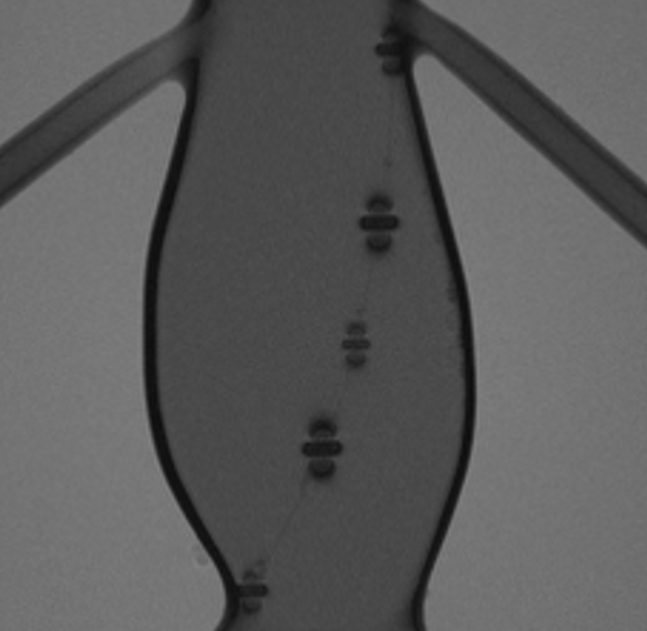
\includegraphics[width=0.6\textwidth]{img/artifact-close.png}
    \caption{Susceptibility artifacts captured with bSSFP sequence at ~4s repetition time and 8mm slice thickness.}
    \label{fig:susceptibility-close}
\end{figure}

To be able to find and detect the susceptibility artifacts from MRI images, computer vision (CV) must be used. It has been well-established that Deep Neural Networks (DNN) are better than standard CV techniques, with some trade offs \cite{computer-vision-cnn-vs-cv}. The trade offs are often considered to be the computing requirements, training time and dataset amount. Nijsink et. al. trained a U-Net deep learning model on manually annotated trainset of 30 images \cite{passive-marker-visibility-and-detection}. Their model was trained to 400 epochs, with random rotation, translation, scale and crop data augmentation techniques. They achieved a great result for 10 validation images, where the median number of correctly detected markers was equal to the number of actual markers.

As an alternative to hand-picking the training data, the artifacts could be artificially simulated. They have a mathematically well-defined magnetic field, as well as the MRI visual response to the field. The susceptibility artifact simulation has been shown in \cite{sim_of_suscept_artifact} and \cite{sus-artifact-subvoxel-sim}.

The main passive tracking technique used for passive guidewires with susceptibility artifacts is "Negative contrast" \cite{active-vs-passive-tracking}.
% https://github.com/MIC-DKFZ/nnUNet

\subsection{Guidewire interventional trauma and safety}
Related work.

\subsection{Problem description and goal}
The goal of this thesis is to provide a solution to the main issues with real-time MRI-based endovascular interventions, which are \textbf{limited/low resolution}, \textbf{guidewire visibility}, \textbf{safety} and \textbf{manual MRI slice alignment} \cite{pmid35420239}. Each of these issues will be addressed by developing a real-time capable imaging software on top of the CathBot robotic platform. \\

\textbf{Limited/low resolution} will be inherently addressed by having a 'real-time' requirement, which is at least 1Hz, or 1 images per second \textcolor{red}{(I could not find any source what is considered real-time in  case of MRI. Best paper was \cite{real-time-mri})}. The image spatial/temporal resolution will be limited, but a CNN dataset will be trained to detect passive guidewire susceptibility artifacts from this resolution. This will relieve the low resolution problem as the guidewire will be digitally shown on the screen.\\

\textbf{Guidewire visibility} will be improved by implementing a CNN detection system for the susceptibility artifacts, and drawing the location of the guidewire based on the location of the artifacts. To streamline the training of the dataset, and allow for future 3D-based detection, a simulated susceptibility artifact will be developed and the dataset will be trained with the simulated artifact.\\

\textbf{Safety} will be improved by incorporating the developed CNN guidewire detection system with the CathBot robotic platform, and building a system to detect if the guidewire is colliding with a blood vessel. For this, a sequence to create a 3D model of the phantom will be created with the help of existing commercial tools such as \cite{slicer}. The 3D model data will be used to find any intersections or close distances with the guidewire.\\

\textbf{Manual MRI slice alignment} \textcolor{red}{(I might not have enough time for this, this section will be developed if all other sections have been completed successfully.)} can be improved by using the commands from CathBot Master device, to predict the next location of the guidewire and move the MRI slice to the appropriate location. For this, the tip of the guidewire must be clearly marked, or detectable by a specifically trained CNN and differentiable from the rest of the guidewire.


\section{Project plan}

\subsection{Simulating susceptibility artifact}
The aim of simulating susceptibility artifacts is to streamline the dataset generation for CNN training. Susceptibility artifacts have a mathematically very well defined magnetic field, and MRI image response. Instead of manually taking pictures of the guidewire with MRI and annotating the artifacts, the artifacts can be simulated and they will look nearly identical to the real-world artifacts. Doing so will greatly simplify and speed up dataset generation for training a CNN. The simulation, and following training dataset will be created with specific settings in reference to Real-Time MRI: bSSFP with ~1s repetition time and slice width of 10mm.

\begin{figure}[h]
    \centering
    \begin{minipage}{0.3\textwidth}
        \centering
        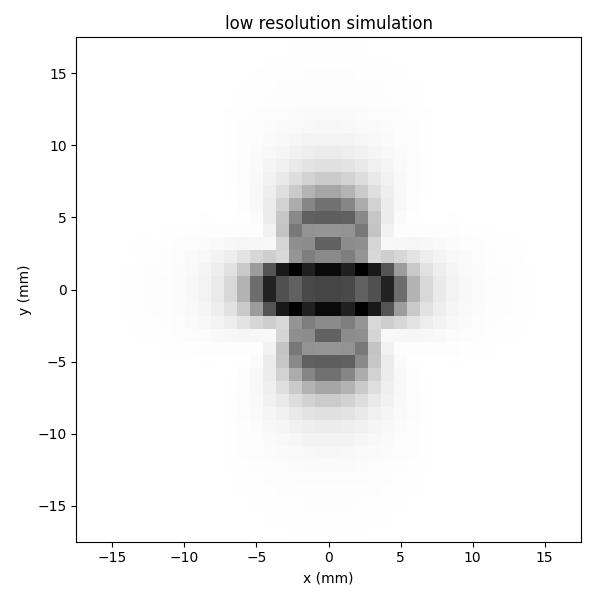
\includegraphics[width=\textwidth]{img/low-resolution-simulation.png}
    \end{minipage}\hfill
    \begin{minipage}{0.3\textwidth}
        \centering
        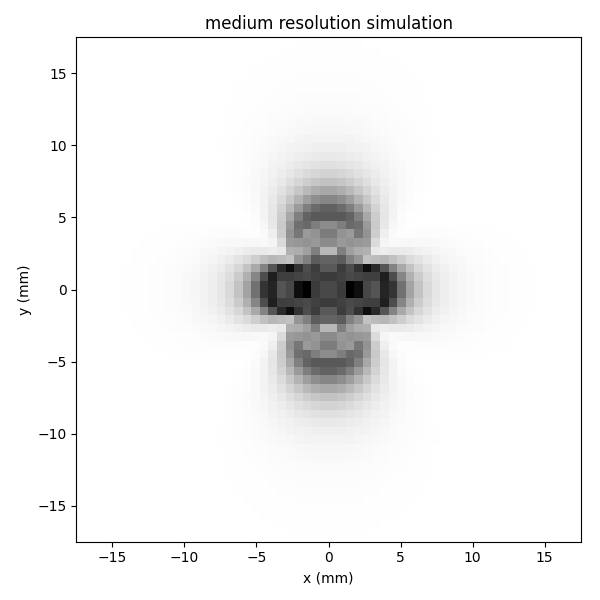
\includegraphics[width=\textwidth]{img/medium-resolution-simulation.png}
    \end{minipage}\hfill
    \begin{minipage}{0.3\textwidth}
        \centering
        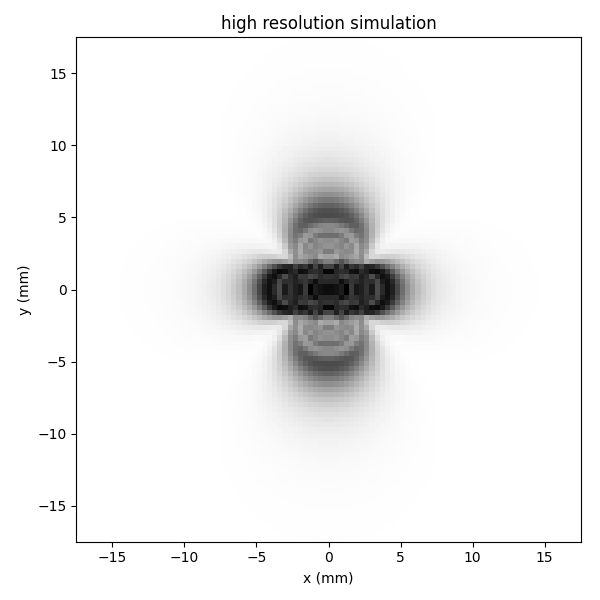
\includegraphics[width=\textwidth]{img/high-resolution-simulation.png}
    \end{minipage}\hfill
    \caption{Susceptibility artifact simulation with different resolution steps}
    \label{fig:sus-representation}
\end{figure}

A proper implementation of the susceptibility artifact simulation should also allow for 3D simulation of the susceptibility artifact, which opens up future work where susceptibility artifacts can be detected in any MRI plane orientation. For the purpose of this thesis, only artifacts that are parallel to the B0 of the MRI (Coronal and Saggital) will be considered.\\
\textbf{Deadline: 22.01.2024}

\begin{figure}[h]
    \centering
    \begin{minipage}{0.45\textwidth}
        \centering
        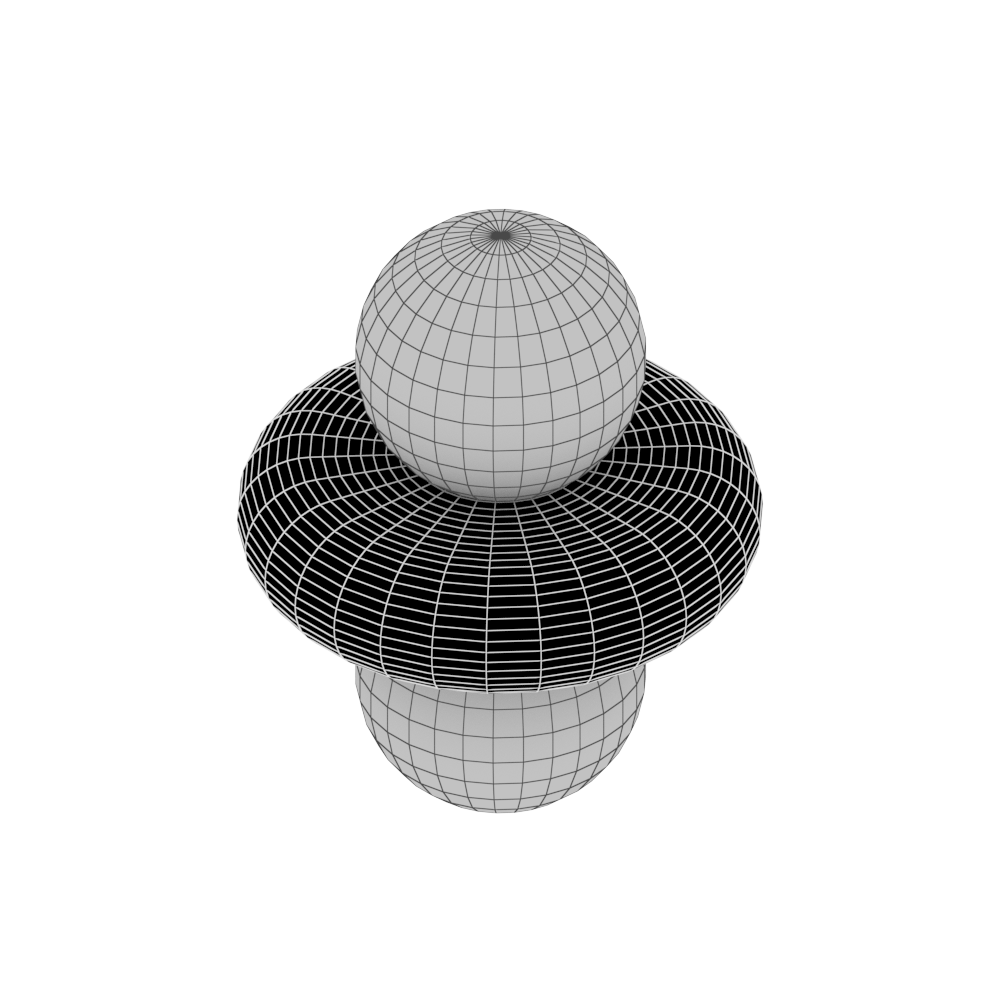
\includegraphics[width=\textwidth]{img/sus-iso-clean.png}
    \end{minipage}\hfill
    \begin{minipage}{0.45\textwidth}
        \centering
        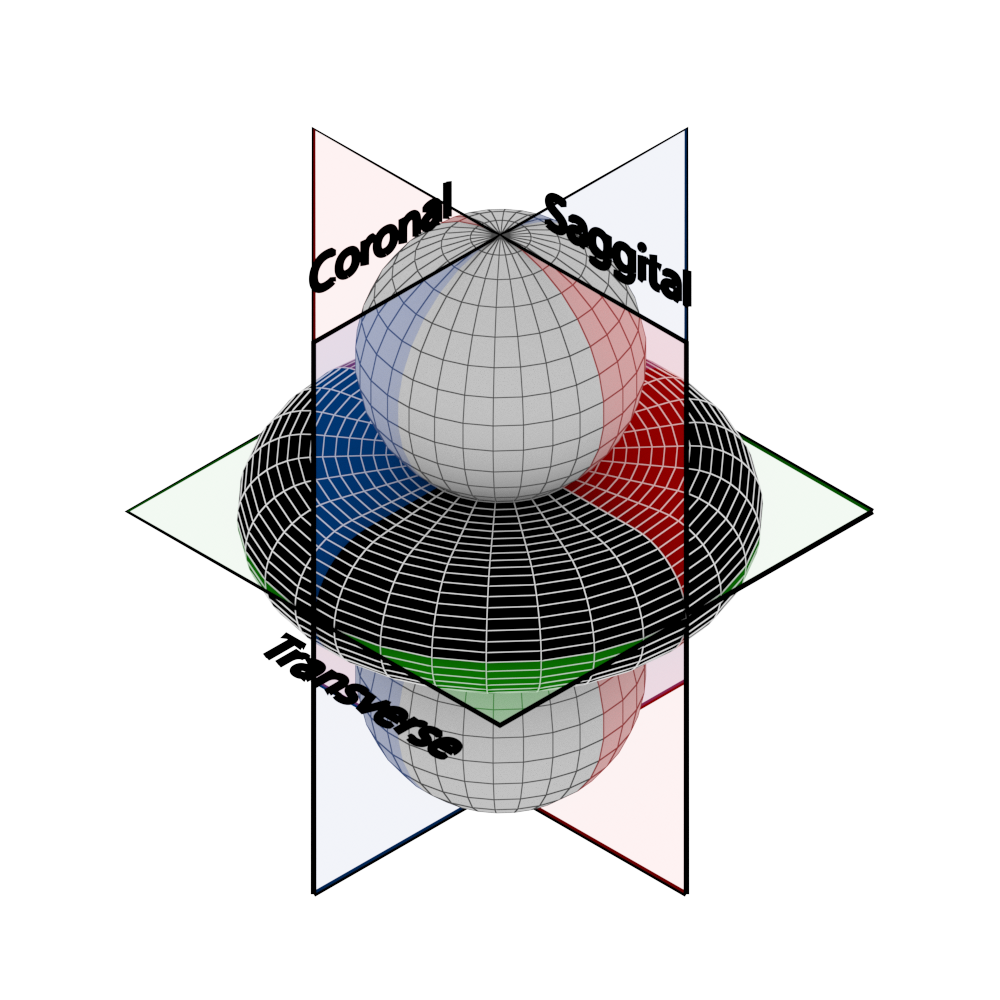
\includegraphics[width=\textwidth]{img/sus-iso.png}
    \end{minipage}\hfill
    \caption{Susceptibility artifact shape 3D representation}
    \label{fig:sus-representation}
\end{figure}

\begin{figure}[h]
    \centering
    \begin{minipage}{0.3\textwidth}
        \centering
        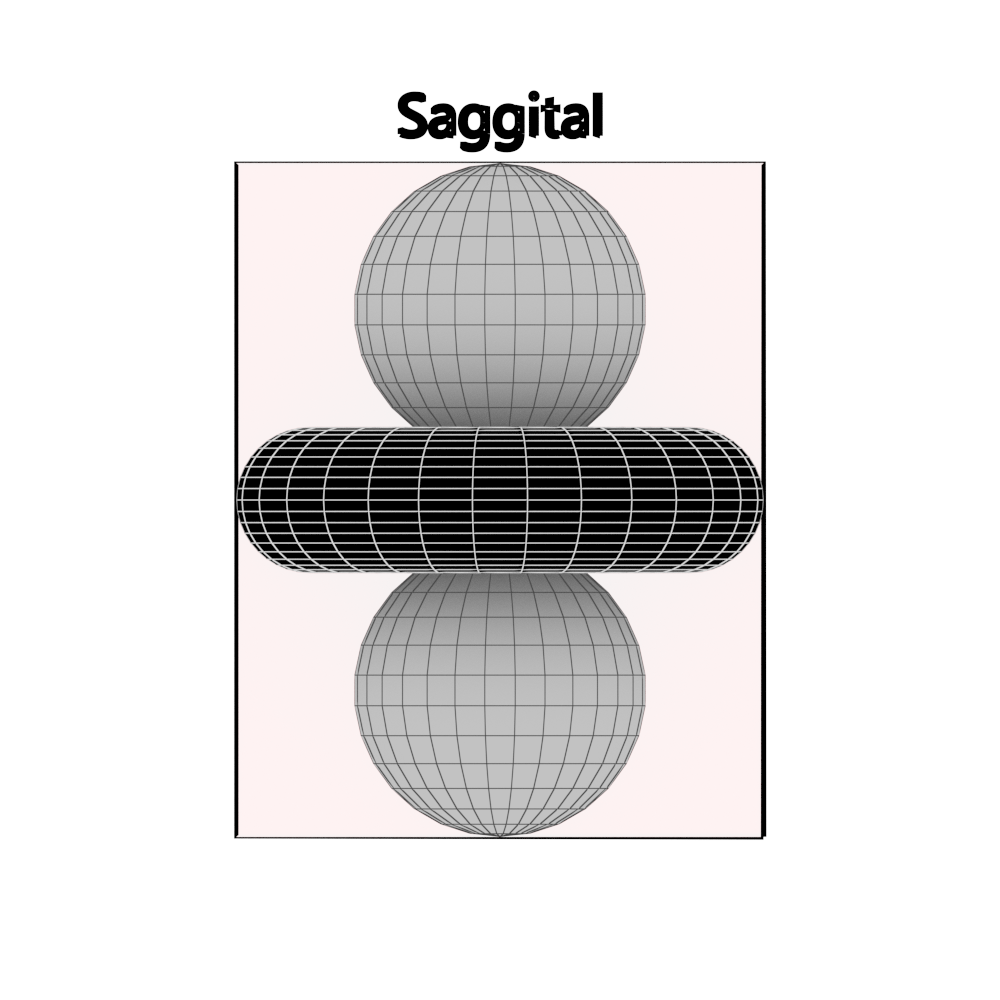
\includegraphics[width=\textwidth]{img/sus-saggital.png}
    \end{minipage}\hfill
    \begin{minipage}{0.3\textwidth}
        \centering
        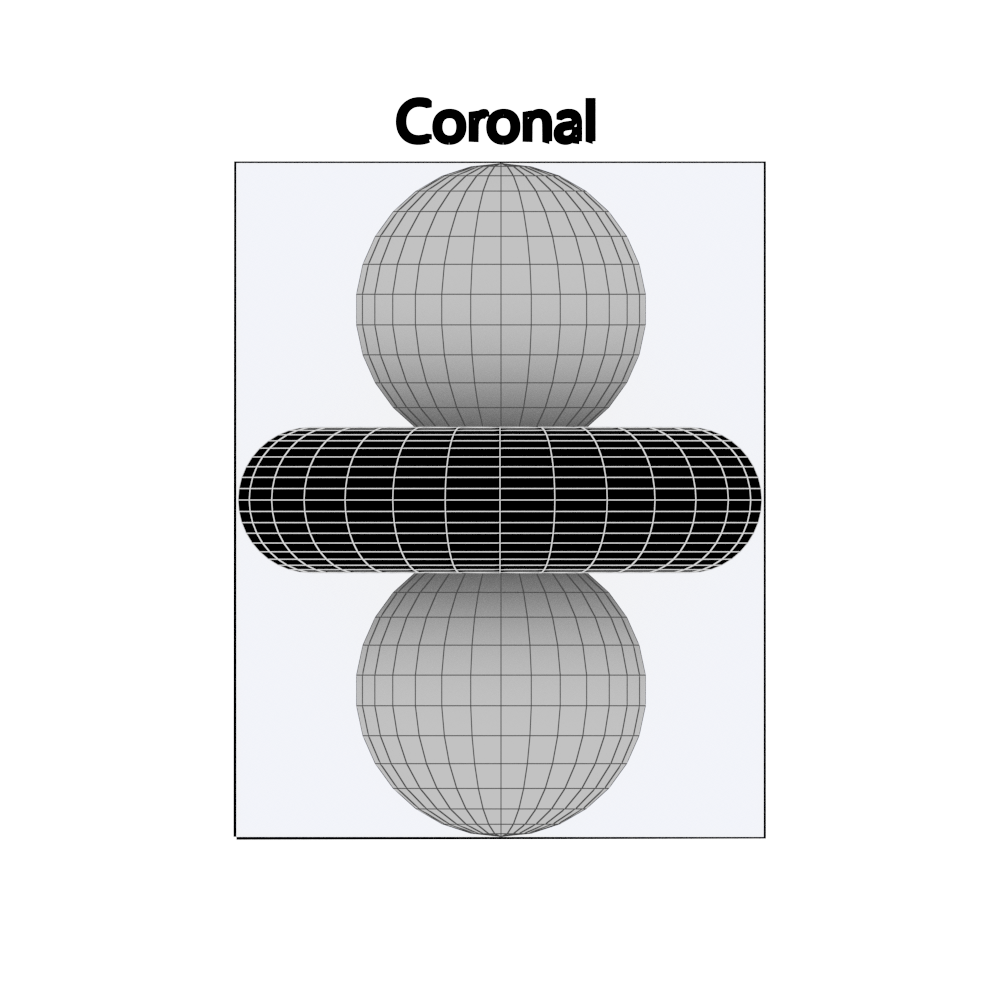
\includegraphics[width=\textwidth]{img/sus-coronal.png}
    \end{minipage}\hfill
    \begin{minipage}{0.3\textwidth}
        \centering
        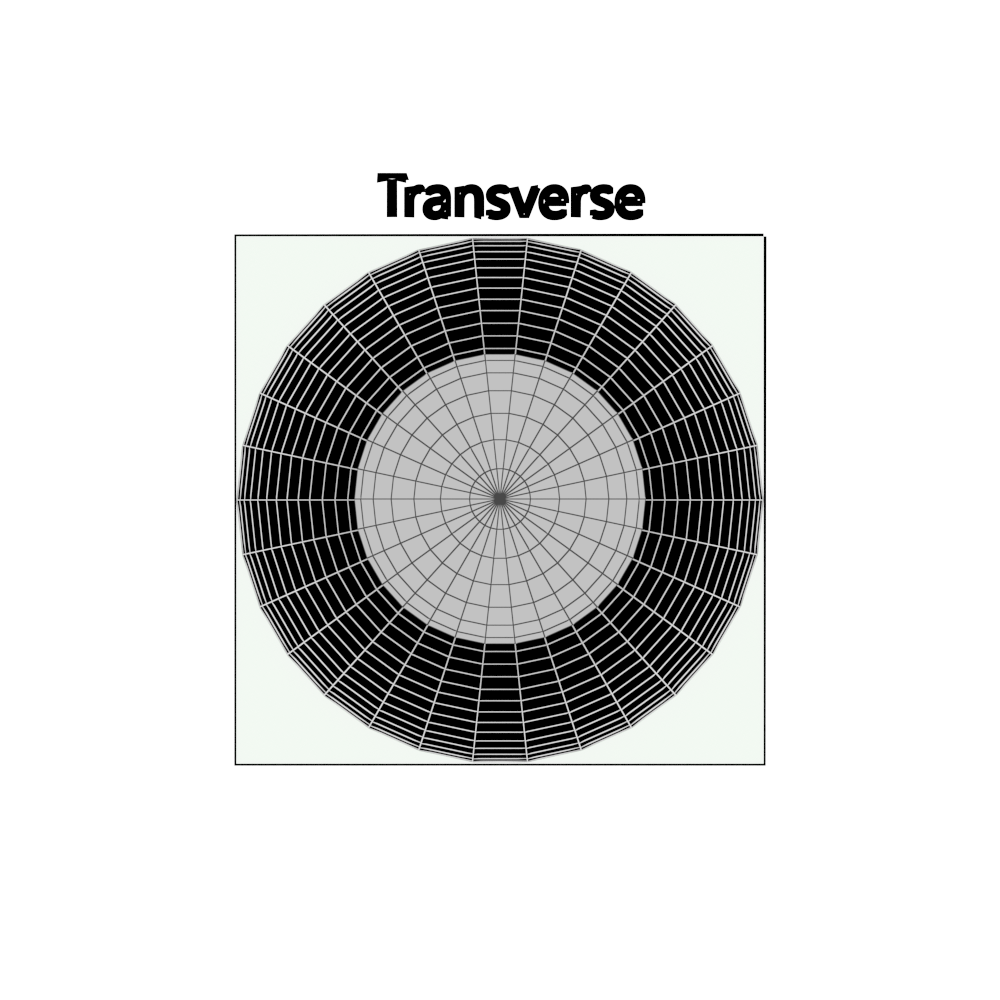
\includegraphics[width=\textwidth]{img/sus-transverse.png}
    \end{minipage}\hfill
    \caption{Susceptibility artifact shape in different MRI planes. Saggital and Coronal planes are parallel with the MR B0 field.}
    \label{fig:sus-representation}
\end{figure}

\newpage

\subsection{Training CNN}
Simulated artifacts will be superimposed on existing MRI datasets, to replicate real-world situations for creating the training dataset. Data augmentation will be used to create variations in size, distance, noise and weakening of contrast to simulate slice thickness changing.\\

Landmark detection and segmentation will be researched and one of these methods will be used to train the CNN. The trained CNN will be a single-class categorization type, which will be trained to specifically identify one type of object from images, which is the susceptibility artifact.\\

The trained CNN model will be used to aid detection of the guidewire under MRI. Each of the susceptibility artifacts will be highlighted and the approximated shape of the guidewire will be drawn on the screen.

If necessary, negative contrast, subtraction and similar imaging methods will be used to simplify the detection in a "ex-vivo" phantom. For the purpose of this project, the most notable issue with subtraction which is sensitivity to motion of the patient and flow artifacts, will be ignored due to the project's time restrictions \cite{passive-tracking-white-marker}.\\
\textbf{Deadline: 01.02.2024}
\newpage
\subsection{Real-Time detection}
The trained CNN and integration with the Siemens Interface will allow to create a pipeline, which can be used to detect the guidewire in real-time. The images from Siemens Interface will be passed into developed software, which shows the passive guidewire marker locations on screen.\\
\textbf{Deadline: 13.02.2024}

\subsection{Creating 3D anatomy from MRI image sequence}
In this phase, existing datasets and tools will be implemented, to digitally map the anatomy scanned using the MRI scanner. The recreation will focus solely on the heart phantom(s) available at RaM. For the purpose of this assignment, existing tools such as Slicer\cite{slicer}  will be used, as developing a novel reconstruction method is not be viable due to the time constraint of this project. The outcome of this phase is software component which is capable of creating a 3D-representation of the heart phantom, relative to the MRI coordinate space.\\
\textbf{Deadline: 15.03.2024}

\subsection{Haptic feedback mechanism on CathBot}
In this phase, a software-based safety layer is implemented on the CathBot platform, which combines all the previously discussed software components to give the operator of the CathBot Master Device more information regarding the positioning of the guide-wire, as well as imposing preventative measures to avoid damaging the patient. The Master Device will give haptic feedback to the operator, when the tip or any other visible guidewire part is dragging or touching the wall of a blood vessel, which could be harmful to the patient.\\
\textbf{Deadline: 03.05.2024}

\newpage
\section{Timeline}
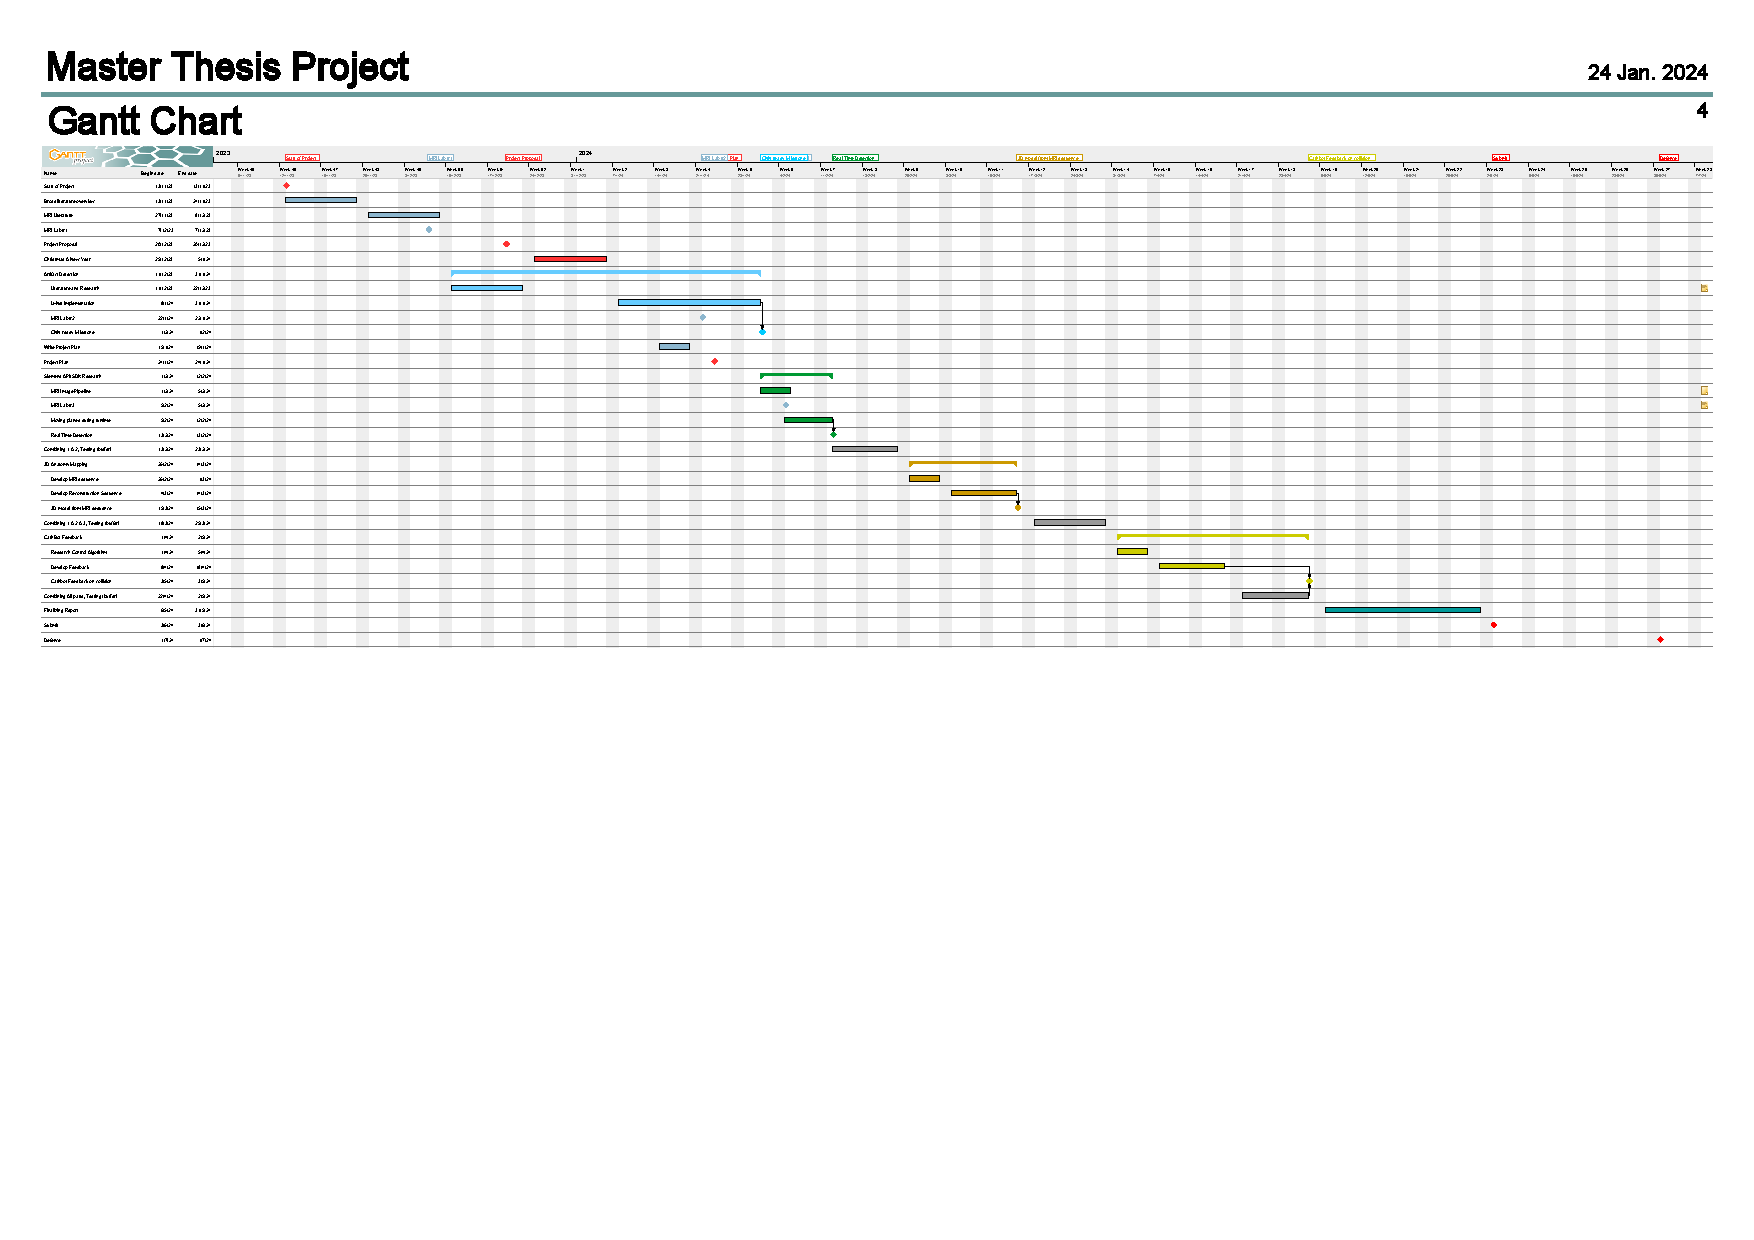
\includepdf[landscape=true]{Thesis-Timeline-24.01.2024.pdf}


\bibliographystyle{alpha}
\bibliography{references}

\end{document}